\documentclass[draftcls,onecolumn,12pt]{IEEEtran}
\usepackage[utf8]{inputenc}
\usepackage[linesnumbered,lined, algoruled]{algorithm2e}
\usepackage{algorithmic,float}
\usepackage{amsmath}
\usepackage{amsthm}
\usepackage{amsfonts}
\usepackage{bm,array}
\usepackage{color,soul}
%\usepackage{epstopdf}
\usepackage[acronym,shortcuts]{glossaries}
\usepackage{graphicx}
\usepackage{graphics}
\makeglossaries
%%% Glossaries/Acronyms


\newacronym{auc}{AUC}{area under the curve}
\newacronym{bs}{BS}{base station}
\newacronym{ce}{CE}{Cross Entropy}
\newacronym{kl}{K-L}{Kullback-Leibler}
\newacronym{llr}{LLR}{log likelihood-ratio}
\newacronym{los}{LOS}{line of sight}
\newacronym{lssvm}{LS-SVM}{least squares SVM}
\newacronym{ml}{ML}{Machine Learning}
\newacronym{mlp}{MLP}{multy-layer perceptron}
\newacronym{mse}{MSE}{Mean Squared Error}
\newacronym{nn}{NN}{Neural Network}
\newacronym{np}{N-P}{Neyman-Pearson}
\newacronym{pdf}{PDF}{probability distribution function}
\newacronym{pso}{PSO}{particle swarm optimization}
\newacronym{rnn}{RNN}{replicator neural network}
\newacronym{roc}{ROC}{receiver operating characteristic}
\newacronym{rss}{RSS}{received signal strength}
\newacronym{svm}{SVM}{Support Vector Machine}
\newacronym{ue}{UE}{user equipment}



\newcommand{\ie}{i.e., }
\newcommand{\wrt}{w.r.t. }
\newcommand{\Exp}[1]{\mathbb{E}\left[#1\right]}

\DeclareMathOperator{\sign}{sign}
\DeclareMathOperator{\E}{E}
\newtheorem{theorem}{Theorem}
\newtheorem{lemma}{Lemma}

\title{Machine learning approaches for position and user authentication in wireless systems}
\author{ }
\date{}

\usepackage[autostyle]{csquotes}



\begin{document}


\maketitle

\sloppy

\begin{abstract}
Physical layer authentication has been proposed as an effective alternative scheme to traditional upper layer-based techniques, such as cryptography, in order to provide a secure authentication scheme. In this paper, we exploit the area specific attenuation values to perform location-based authentication, i.e. granting access to the network only to users located in a pre-defined area. We first exploit the \ac{np} optimal criterion to formulate the problem as hypothesis testing. Secondly, we implement the authentication system by exploiting to \ac{ml} techinques, namely the \acp{nn} and the \ac{svm}. We then show how the output of the \ac{nn} trained with two different loss functions, namely the \ac{mse} and the \ac{ce}, are related to \ac{np} optimal hypothesis testing. The same result has been derived for \ac{svm}. By introducing a realistic channel model we then show that the proposed \ac{nn} implementation of the authentication system is convenient respect to \ac{np}. The problem of network planning is hence addressed and lastly we propose a possible atteck strategy.
\end{abstract}

\begin{IEEEkeywords}
Physical layer security, authentication, neural network, auto-encoder, support vector machine
\end{IEEEkeywords}

\glsresetall

\section{Introduction}
Traditional authentication systems are based on upper-layer techniques such as cryptography. However, as the network latency requirement becomes stricter, the timely sharing of security keys in large and dense networks may not be supported by this type of networks. This is further complicated by the computational cost of key generation and detection. On the other hand, as the computational power of devices grows, the time spent in cracking a digital security key may be remarkably shortened \cite{Wang-16}. Physical layer techniques have been proposed as an alternative to digital key generation. These techniques exploit properties of the communication channel such as the \ac{rss} to distinguish radio transmitters. In this paper, we exploit area specific attenuation values to distinguish between a legitimate and non-legitimate area, implementing in such a way a location-based authentication system.

Traditional detection systems are based on \ac{np} lemma which rejects a hypothesis in favor of the other based on the comparison of the likelihood ratio with a suitably chosen threshold value. An example application of this criterion is \cite{Baracca-12}, where the \ac{np} framework has been exploited to implement an authentication system suited for multiple wiretap channels with correlated fading. A generalization of the \ac{np} framework is presented in \cite{Xiao-09}, where physical layer authentication is performed over a Rayleigh fading channels and detection is implemented via generalized likelihood ratio test. A further example is \cite{Pan-17}, where \ac{ml} algorithms have been exploited in order to find the best threshold needed for hypothesis testing.

However, the knowledge of the channel statistics as well as its model may not be available. In this context, the computation of the likelihood functions needed for hypothesis testing can be estimated by the available data but may not be accurate. \ac{ml} techniques have been introduced as an alternative method to perform user authentication without requiring prior knowledge of the channel statistics. This issue has been tackled by \cite{xiao-2018}, where no assumption is made on the channel model and logistic regression has been proposed as alternative to hypothesis testing. In \cite{Wang-17}, a feed-forward neural network receives as input the Euclidean distance between successive channels and the Pearson coefficient as feature space to perform authentication. 
%
 \hl{Literature overview on SVM to be added $(https://www.researchgate.net/publication/279246263_Robust_indoor_localization_and_tracking_using_GSM_fingerprints$
; $https://ieeexplore.ieee.org/abstract/document/7037452/$)}.

In this paper, we compare the performance of the authentication system based on \ac{np} optimality criterion, henceforth referred to as \ac{np} detector, with \ac{ml} based approaches. In particular, we investigate the performance of the \ac{ml}-based authentication systems implemented via \ac{nn} and via \ac{svm}. We consider two different \ac{nn} architectures: the multi-layer perceptron and the auto-encoder. For the multi-layer perceptron, we investigate two loss functions: the \ac{ce} and the \ac{mse}. We show that both loss functions guarantee the same performance of the optimal \ac{np} detector in terms of true positive and false negative rate. Further details about the architectures and the training objective function will be discussed in section \ref{sec:nn}.

In section \ref{sec:auto} we consider the problem of performing hypothesis testing when samples from one of the two classes are available and no information on the other class can be obtained. The auto-encoder \ac{nn} is proposed as solution for this problem.

In section \ref{sec:svm}, we introduce the \ac{svm} and we show how it can be exploited to implement an authentication system. Furthermore, we show that the output of such a system is related to the \ac{np} lemma.

In sections \ref{sec:res_los} and \ref{sec:res_nLos} we confirm via numerical results the theoretical parts of the previous section and investigate the performance of the different implementations of the authentication system.

In section \ref{sec:bsPos}, we consider the problem of network planning, i.e., find the optimal positions of the \acp{bs} needed to implement the authentication system. We show that the \ac{nn} can be exploited in the optimization procedure.

The contribution of this paper can be summarized as follows:
\begin{itemize}
    \item We propose an implementation of a physical layer-based location authentication system which exploits \ac{ml} techniques to perform hypothesis testing;
    \item We show that the performance obtained with this \ac{ml} techniques are optimal in a \ac{np} sense;
    \item We compare different \ac{ml} techniques and show how these can be exploited to implement different levels of the authentication system, from the planning of the network to authentication and attacks.
\end{itemize}

The following notation will be used throughout the paper: bold letters $\bm{x}$ refer to vectors, whereas capital bold letters $\bm{H}$ refer to matrices, $\mathbb{E}[]$ denotes the expected value, $e_i$ denotes the all zero vector except for component $i$ which is equal to $1$ and $(\cdot)^T$ denotes the transpose.

\section{System Model}
Consider a network with $N_{\rm bs}$ \acp{bs}, where \ac{bs} $n$, $n=1,...,N_{\rm bs}$, is located in position $\bm{x}_{\rm bs}^{(n)} =(X_{\rm bs}^{(n)},Y_{\rm bs}^{(n)})$, where entries represent respectively the $x$ and $y$ coordinates. 

Consider a \ac{ue} transmitting with power $P_{\rm tx}$. The received power at the $n^{\rm th}$ \ac{bs} is
\begin{equation}
    P_{\rm rc}^n[dB]= P_{\rm tx}[dB] -  a^{(n)}[dB],
\end{equation}
where $a^{(n)}$ is the attenuation incurred by the transmitted signal to \ac{bs} $n$. Assuming that the transmitting power of each \ac{ue} is known, the \ac{bs} can compute the attenuation value $a^{(n)}$. As signals transmitted from different locations incur to different attenuation we exploit such values to implement the authentication system.

We propose two models for the attenuation coefficient $a^{(n)}$. Consider a \ac{ue} located in position $\bm{x}_{\rm ue}=(X_u,Y_u)$. Let us define the distance between the \ac{ue} and the \ac{bs} as
\begin{equation}
    L(\bm{x}_{\rm ue},\bm{x}_{\rm bs}^{(n)}) = \sqrt{(X_{\rm bs}^{(n)}-X_u)^2+(Y_{\rm bs}^{(n)}-Y_u)^2}.
\end{equation}
When considering \ac{los} links the path loss is modelled as
\begin{equation}\label{eq:los}
    P_{\rm LOS}^{(n)}[dB] = 20\log_{10}\left(\frac{f 4\pi L(\bm{x}_{\rm ue},\bm{x}_{\rm bs}^{(n)})}{c}\right),
\end{equation}
where $f$ is the carrier frequency and $c$ is the speed of light.
We refer to the \textit{\ac{los} scenario} the case where $a^{(n)}=P_{\rm LOS}$.

When considering non-\ac{los} links path loss is defined as
\begin{equation}
    P_{\rm non-LOS}^{(n)}[dB] = 40\log10\left (\frac{L(\bm{x}_{\rm ue},\bm{x}_{\rm bs}^{(n)})}{10^3}\right ) + 21\log10\left(\frac{f}{10^6}\right) + 80;
\end{equation}

The shadowing term $s \sim \mathcal{N}(0,\sigma_s^2)$ is modelled as a zero mean $\sigma_s^2$ variance Gaussian random variable. We will refer to the \textit{full scenario} when considering both \ac{los} non-\ac{los} links, shadowing effects and fading. In the full scenario the attenuation toward the $n^{\rm th}$ \ac{bs}, due to the shadowing effects, is modelled as normal random variable with zero mean and variance
\begin{equation}\label{eq:rss}
    \sigma_f^2(n) = P_l^{(n)}n-4,34s,
\end{equation}
and hence the attenuation coefficient due to fading is modelled as
\begin{equation}\label{eq:fade}
a^{(n)}[dB]= \mathcal{N}(0,\sigma_f^{-2}(n)).
\end{equation}

Let us denote as $\mathcal{A}_0$ the legitimate area, i.e., where \acp{ue} are allowed to access the network and as $\mathcal{A}_1$ the area where \acp{ue} are not allowed to access the network. Assume that $\mathcal{A}_0$ is a sub-region of $\mathcal{A}_1$. Let us denote as $|\mathcal{A}_{0}|$ the area in $m^2$ of the legitimate region and as $|\mathcal{A}_{1}|$ the area in $m^2$ of the non-legitimate region.
Since $\mathcal{A}_0 \subset \mathcal{A}_1$ the size of the overall area coincides with $|\mathcal{A}_1|$. 

\section{Location authentication}\label{sec:auth}
Consider a location authentication system based on physical layer information. In such a system, the legitimate user, traditionally referred to as Alice, sends a message to a central system, traditionally referred to as Bob, that is in charge of authenticating it. The process is divided in two phases: location association and location verification. In location association phase, Alice sends a message $x$ to Bob through a secure channel $h$. Bob associate the channel $h$ to Alice and what Bob expects is that each successive message coming from Alice will go through a channel that is very similar to $h$. During the location verification phase, Bob receives a message from an unknown user and estimates a channel $\hat{h}$: if $\hat{h}$ is very similar to $h$, then Bob can conclude that the message comes from Alice. Otherwise, nothing can be said on the identity of the transmitter and the message is considered non-secure.

We exploit this two-step authentication procedure in order to grant access to the network only to users located in area $A_0$. Let us define the attenuation vector $\bm{a}=[a^{(1)},...,a^{(N_{\rm bs})}]$, whose $n^{\rm th}$ entry is the attenuation value measured at the $n^{\rm th}$ \ac{bs} for the current message. During the location association phase, we collect attenuation vectors from both area $A_0$ and area $A_1$ in order to create the sets $\mathcal{S}_0$ and $\mathcal{S}_1$ of the attenuation vectors of the two areas. The idea is that different areas are associated to different attenuation vectors and, if $N_{\rm bs}$ is sufficiently large, we can discriminate area based on attenuation vectors. During the location verification phase, the system compares the current attenuation vector, i.e., the one associated to the current message, with those associated to area $A_0$ and if a match is detected the user is granted access to the network.

This problem has a straightforward formulation as an hypothesis testing problem. Let us define the two hypothesis: a) hypothesis $\mathcal{H}_0$, i.e., the user is transmitting from area $\mathcal{A}_0$; b) hypothesis $\mathcal{H}_1$, i.e., the user is transmitting from area $\mathcal{A}_1$.

Given the attenuation vector $\bm{a}$ we want to determine which of the two hypothesis is more likely to be true in order to implement the aforementioned authentication system. 
We exploit the Neyman-Pearson lemma to test the hypothesis. Let us define the \ac{llr}
\begin{equation}\label{eq:lr}
    \mathcal{L}=\log\left(\frac{p(\bm{a}|\mathcal{H}_0)}{p(\bm{a}|\mathcal{H}_1)}\right),
\end{equation}
where $p(\bm{a}|\mathcal{H}_{\cdot})$ is the probability of measuring the attenuation vector $\bm{a}$ given that hypothesis $\mathcal{H}_\cdot$ is verified. According to the \ac{np} lemma, the most powerful test is the one that compares the value $\mathcal{L}$ with a threshold value $\Lambda$ in order to choose the more likely hypothesis. Let us define two error probabilities: $P_{\rm FA}$ as the false alarm probability, i.e. the probability $P(\hat{\mathcal H} = \mathcal H_1 | \mathcal H_0)$ that a legitimate user is classified as non-legitimate; $P_{\rm MD}$ as the mis-detection probability, i.e., the probability $P(\hat{\mathcal H} = \mathcal H_0 | \mathcal H_1)$ that a non-legitimate user is classified as legitimate. The \ac{np} lemma ensures that, given a false alarm probability value the minimum mis-detection probability is obtained by choosing
\begin{equation}
    \begin{cases}
    \mathcal{H}_1 \quad\text{if} \quad \mathcal{L} \le \Lambda \\
    \mathcal{H}_0  \quad\text{if} \quad \mathcal{L} > \Lambda.
    \end{cases}
\end{equation}

This method ensures that the performance of the authentication system are optimal. However the statistics needed to compute the \ac{llr} (\ref{eq:lr}) are not always available. A numerical approximation can be obtained in certain cases, but we will show  that this requires a large data-set to get a good approximation. In the following sections we introduce different \ac{ml} techniques that will be exploited to implement the authentication system without requiring a-priori knowledge of the channel statistics.

\section{Neural network overview}\label{sec:nn}

A \ac{nn} is a function of the type $f:\mathbb{R}^N \to \mathbb{R}^O$ which maps a set of $N$ real values into $O$ real values. A \ac{nn} is identified by three types of layer: the input layer, the hidden layers, and the output layer. This architecture is also known as \ac{mlp}

Let us consider a \ac{nn} with $L-1$ layers and denote as $N^{(\ell-1)}$ is the size of the $(\ell-1)^{\rm th}$ layer. The output of the $n^{\rm th}$ neuron of the $\ell^{\rm th}$ layer is
\begin{equation}\label{eq:nonLin}
y_n^{(\ell)} = \sigma\left( \bm{w}_n^{(\ell -1)}\bm{y}^{(\ell-1)}+b_n^{(\ell)} \right),
\end{equation}
i.e., a mapping via an activation function $\sigma$ of the weighted linear combination with weights $\bm{w}_n^{(\ell -1)}\in \mathbb{R}^{1\times N^{(\ell-1)}}$ of the outputs $\bm{y}^{(\ell-1)} \in \mathbb{R}^{N^{(\ell-1)} \times 1 }$ of the previous layer plus a bias $b_n^{(\ell)} \in \mathbb{R}^{N^{(\ell-1)} \times 1 }$. The types of layer are characterized by the weights and the activation functions to be used. In the input layer each neuron corresponds to a single value of the input vector, hence , by defining as the layer $0$ the input layer, we have $\bm{w}_n^{(0)}= e_n$. The activation function of the input layer is the identity function.

The weights of each layer are updated by means of a supervised learning algorithm which feed to the network a set of input values and the corresponding labels, i.e. known output values, such that the input values are mapped to the corresponding output labels. The activation function of the hidden layers is the sigmoid function
\begin{equation}
\sigma(x) = \frac{1}{1-e^{-x}},
\end{equation}
whereas the activation function of the output layer is a $\tanh^{-1}$ function
\begin{equation}
\tanh^{-1}(x) = \frac{1}{2} \left( \frac{1+x}{1-x} \right).
\end{equation}


Consider a network with $N_{\rm BS}$ \acp{bs}. Since the information available at \ac{bs} $n$ is the attenuation value $a_n$ we use the attenuation vector $\bm{a}$ as input of the \ac{mlp}. The input layer will be hence composed by $N_{\rm BS}$ neurons. The objective is to train a \ac{mlp} with a single output neuron whose value is used for hypothesis testing. 

In the next sections we investigate the effects of training the \ac{mlp} with two different loss functions: the \ac{mse} and the \ac{ce}.

\subsection{ MSE training}
Consider a set of training attenuation vectors $\bm{a}^{(i)} \, , \, i=1,...,S$ with target output $\theta^{(i)} \, , \, i=1,...,S $ where $\theta^{(i)}$ is equal to $1$ if $\bm{a}^{(i)}$ has been generated form a user located in area $\mathcal{A}_0$ whereas $\theta^{(i)}=-1$ if $\bm{a}^{(i)}$ has been generated form a user in $\mathcal{A}_1$. Let us define as $\bm{\theta}_{\rm MSE}$ the vector of target values, i.e., $\bm{\theta}_{\rm MSE}=[\theta^{(1)},...,\theta^{(S)}]$.

Let us define as $\tilde{\bm{\theta}}_{\rm MSE}$ the vector of the output values of the \ac{mlp}, whose $i^{\rm th}$ component is the output of the \ac{mlp} obtained with the $i^{\rm th}$ training vector. The \ac{mlp} training is performed via gradient descent minimizing the \ac{mse}, defined as
\begin{equation}
MSE = \mathbb{E}[||\tilde{\bm{\theta}}_{\rm MSE}-\bm{\theta}_{\rm MSE}||^2].
\end{equation}

Since the output of the neural network $\theta^{(i)}$ is a continuous value in ${-1,1}$, in order to perform classification, a suitable threshold value $\lambda$ must be chosen, such that the input vector $\bm{a}^{(i)}$ is classified as
\begin{equation}
\bm{a}^{(i)} \in
\begin{cases}
\mathcal{A}_0 \, \text{if} \, \theta^{(i)} > \lambda \\
\mathcal{A}_1 \, \text{if} \, \theta^{(i)} \le \lambda, 
\end{cases}
\end{equation}
where $\bm{a}^{(i)} \in \mathcal{A}_.$ denotes that the attenuation vector $\bm{a}^{(i)}$ has been generated from a \ac{ue} located in area $\mathcal{A}_.$.

The test to be performed is hence similar to the one performed by the \ac{np} detector. In the next section we show the relation that exists between \ac{mse} training and the optimal hypothesis testing. 

\subsection{MSE training connection with N-P lemma}
In the previous section we showed that a \ac{nn} implements a function $f(\bm{a},\bm{W})$, where $\bm{a}$ is the vector of input parameters and $\bm{W}$ is the matrix whose $\ell{\rm th}$ column is obtained by stacking the vector of weights $\bm{w}_n^{(\ell)}$ and bias $b_n^{(\ell)}$ of each neuron of the $\ell{\rm th}$ layer. In this section we are going to prove the following theorem:
\begin{theorem}
\label{th:nn_np}
Consider a \ac{nn} with perfect training and a sufficient number of parameters such that training reaches a global minimum. Then the classificator obtained by training the \ac{nn} via \ac{mse} is equivalent to the classificator obtained via \ac{np} lemma.
\end{theorem}
\begin{proof}
Consider the function $f(\bm{a},\bm{W})$ implemented by the \ac{nn} and the Bayes optimal discriminant function
\begin{equation}
g_0(\bm{a}) = \mathbb{P}(\mathcal{H}_0|\bm{a}) - \mathbb{P}(\mathcal{H}_1|\bm{a}).
\end{equation} 
The \ac{mse} obtained by a \ac{nn} performing classification with target outputs ${-1,1}$ for the two hypothesis can be written as \cite{Ruck-90}
\begin{equation}\label{eq:mseAs}
E_t(\bm{W}) = \mathbb{E} \left\{ \left( f(\bm{a},\bm{W} - g_0(\bm{a}) \right)^2 \right\} + \left \{1-\mathbb{E}[g_0(\bm{a})]^2\right \}.
\end{equation}
The \ac{nn} training problem is solved by minimizing $E_t(\bm{W})$ respect to the parameters $\bm{W}$ and we notice that the second term in (\ref{eq:mseAs}) does not depend on $\bm{W}$.
From \cite{Ruck-90}, when the number of parameters goes to infinity, we obtain
\begin{equation}\label{eq:bayesDisc}
f(\bm{a},\bm{W}) \approx \mathbb{P}(\mathcal{H}_0|\bm{a}) - \mathbb{P}(\mathcal{H}_1|\bm{R}). 
\end{equation}
By recalling that $\mathbb{P}(x|y)=\mathbb{P}(y|x)\mathbb{P}(x)/\mathbb{P}(y)$ we can write
\begin{equation}
g_0(\bm{a}) = \frac{{\mathbb P}(\bm{a}|\mathcal H_0){\mathbb P}(\mathcal H_0) - {\mathbb P}(\bm{a}|\mathcal H_1){\mathbb P}(\mathcal H_1)}{\mathbb P(\bm{a})},
\end{equation}
which in turn can be written as
\begin{equation}
g_0(\bm{a}) = \frac{{\mathbb P}(\bm{a}|\mathcal H_0){\mathbb P}(\mathcal H_0) - {\mathbb P}(\bm{a}|\mathcal H_1){\mathbb P}(\mathcal H_1)}{{\mathbb P}(\bm{a}|\mathcal H_0){\mathbb P}(\mathcal H_0) + {\mathbb P}(\bm{a}|\mathcal H_1){\mathbb P}(\mathcal H_1)}.
\end{equation}
By imposing a threshold $\lambda$ on $g_0(\bm{a})$ and reorganizing we obtain
\begin{equation}
\frac{{\mathbb P}(\bm{a}|\mathcal H_0)}{{\mathbb P}(\bm{a}|\mathcal H_1)}>   \frac{{\mathbb P}(\mathcal H_1)}{{\mathbb P}(\mathcal H_0)} \frac{1 + \lambda}{1-\lambda} = \lambda^*,
\end{equation}
which is equivalent to the \ac{np} criterion.
\end{proof}

\subsection{CE training}
Consider the training attenuation vectors set $\bm{a}^{(i)}$, $i=1,...,S$ with target output vector $\bm{\theta}^{\rm CE}$, where the $i^{\rm th}$ component is equal to $1$ if $\bm{a}^{(i)}$ has been generated form a user located in area $\mathcal{A}_0$ whereas $\theta_i=0$ if $\bm{a}^{(i)}$ has been generated form a user in $\mathcal{A}_1$. Let us define as $\tilde{\bm{\theta}}^{\rm CE}$ the vector whose $i^{\rm th}$ component $\tilde{\theta}_i^{\rm CE}$ is the output of the \ac{nn} obtained with the $i^{\rm th}$ training vector. The \ac{nn} training is performed via gradient descent minimizing the \ac{ce} defined as
\begin{equation}\label{eq:ce}
CE = -\sum_{i=1}^{S}\left(\tilde{\theta}_i^{\rm CE}log\left(\theta_i^{\rm CE}\right)+\left(1-\tilde{\theta}_i^{\rm CE}\right)log\left(1-\theta_i^{\rm CE}\right) \right).
\end{equation}
In this case the output of the \ac{nn} is a continuous value between $0$ and $1$ and a suitable threshold value must be chosen in order to assign label $0$ or $1$ to the considered input vector.

Comparison with a threshold is the key step of the \ac{np} lemma and we notice that this is also required when performing \ac{ce} training. In the next section we show how the two methods are related.

\subsection{CE training connection to N-P lemma}
When training is performed with \ac{ce} loss function the output of the \ac{nn} represents the probability $\mathbb{P}(\mathcal{H}_0|\bm{a}^{(i)})$ of being in hypothesis $\mathcal{H}_0$ given that the attenuation vector is $\bm{a}^{(i)}$ \cite{Bishop2006}, i.e.,
\begin{equation}
    f(\bm{a}^{(i)},\bm{W}) \approx \mathbb{P}(\mathcal{H}_0|\bm{a}^{(i)}),
\end{equation} 
where $\bm{W}$ is the matrix whose $\ell{\rm th}$ column is obtained by stacking the vector of weights $\bm{w}_n^{(\ell)}$ and bias $b_n^{(\ell)}$ of each neuron of the $\ell{\rm th}$ layer.

In this section we prove the following
\begin{theorem}
\label{th:nn_np2}
Consider a \ac{nn} with perfect training and a sufficient number of parameters such that the training reaches a global minimum. Then the classificator obtained by training the \ac{nn} via \ac{ce} is equivalent to the classificator obtained via \ac{np} lemma.
\end{theorem}
\begin{proof}
Since we are considering a two class classification problem the probability $\mathbb{P}(\mathcal{H}_1|\bm{a}^{(i)})$, i.e., the probability of being in hypothesis $\mathcal{H}_1$ given that the attenuation vector is $\bm{a}^{(i)}$, is obtained as
\begin{equation}
    \mathbb{P}(\mathcal{H}_1|\bm{a}^{(i)}) = 1- \mathbb{P}(\mathcal{H}_0|\bm{a}^{(i)}).
\end{equation}
By imposing a threshold on the output of the \ac{nn} we obtain
\begin{equation}
    f(\bm{a}^{(i)},\bm{W}) \approx \mathbb{P}(\mathcal{H}_0|\bm{a}^{(i)}) > \lambda,
\end{equation}
which can be rewritten as
\begin{equation}
    2\mathbb{P}(\mathcal{H}_0|\bm{a}^{(i)})-1 > \hat{\lambda}
\end{equation}
\begin{equation}
    \mathbb{P}(\mathcal{H}_0|\bm{a}^{(i)})-(1-\mathbb{P}(\mathcal{H}_0|\bm{a}^{(i)})) > \hat{\lambda}
\end{equation}
\begin{equation}
    \mathbb{P}(\mathcal{H}_0|\bm{a}^{(i)})-\mathbb{P}(\mathcal{H}_1|\bm{a}^{(i)}) > \hat{\lambda}.
\end{equation}
We hence obtained the same formulation of (\ref{eq:bayesDisc}) and, by following the same steps of the proof of theorem 1 we see that imposing a threshold on the output of the \ac{ce}-trained \ac{nn} is equivalent of performing hypothesis testing with \ac{np} lemma.
\end{proof}

\section{Replicator neural network}\label{sec:auto}
In this section we consider the case where discrimination between the two areas $\mathcal{A}_0$ and $\mathcal{A}_1$ is performed based on data generated only from the authentic region, i.e., the available attenuation vectors $\bm{a}^{(i)}$ used for training are generated from \acp{ue} located in $\mathcal{A}_0$. This type of problem is usually referred to as \textit{one-class classification}. 

In order to solve this problem we exploit a \ac{nn} that implements a \textit{\ac{rnn}}, i.e., a network that is trained to: a) convert high-dimensional inputs to low-dimensional codes in the hidden layer; b) reconstruct the high-dimensional input at the output layer from the low-dimensional codes of the hidden layer \cite{Hinton-2006}.

Consider a set $\mathcal{U}$ and a set of vectors $\mathcal{V} \in \mathcal{U}$. If this vectors are used for training the auto-encoder, each new input vector $\bm{v} \in \mathcal{U}$ is mapped at the output with a small reconstruction error, whereas each input vector $\bm{v} \notin \mathcal{U} $ is mapped at the output with a large reconstruction error.

The capacity of the auto-encoder to replicate only certain values at the output is due to the fact that the hidden layer is able the extract the features of the set $\mathcal{U}$ used for training. This is particularly true when the size of the hidden layer is lower than the size of the input layer, i.e. when $M<N$ \cite{Bourlard-88}.

Consider an \ac{rnn} with three layers, i.e., a size $N$ input layer, a size $M$ hidden layer and a size $N$ output layer.  The function mapping the input layer to the hidden layer is of the form (\ref{eq:nonLin}), whereas the non-linearity is removed when mapping the hidden layer to the output layer. This is due to the fact that the network must reconstruct real values and hence the output shall not be limited in a range of values. 

The $n^{\rm th}$ output $y_n^{(o)}$ of the output layer is obtained from
\begin{equation}
    y_n^{(o)}= \bm{w}_n^{(o)}\bm{y}^{(h)}+b_n^{(h)}
\end{equation}
where $\bm{w}_n^{(o)}$ is the $1\times M$ vector of weights assigned to the $n^{\rm th}$ output, $\bm{y}^{(h)}$ is the $M\times 1$ vector of the outputs of the hidden layer and $b_n^{(h)}$ is the $n^{\rm th}$ bias of the hidden layer.


We here exploit the \ac{rnn} to implement the authentication system described in section \ref{sec:auth}. 

Consider the input attenuation vector $\bm{a}$ and its replicated value $\hat{\bm{a}}$ at the output of the auto-encoder after training.
Let us define the reconstruction error
\begin{equation}\label{eq: rec err}
    \epsilon = \frac{1}{N}\sum_{i=1}^{N}|a_i-\hat{a}_i|^2,
\end{equation}
where $a_i$ denotes the $i^{\rm th}$ component of the vector. The authentication system performs a test comparing the reconstruction error $\epsilon$ with a threshold value $\gamma$ and chooses 
\begin{equation}
\bm{a} \in
\begin{cases}
\mathcal{A}_0 \, \text{if} \, \epsilon < \gamma \\
\mathcal{A}_1 \, \text{if} \, \epsilon \ge \gamma. 
\end{cases}
\end{equation}
\section{Support Vector Machine}\label{sec:svm}
A \ac{svm} \cite{Bishop2006} is a supervised learning model that can be used for classification and regression. We focus here on binary classification, \ie given the input attenuation vector $\mathbf{a}^{(i)} \in \mathbb{R}^N$ the \ac{svm} returns $y_i = 1$ if $\mathbf{a}^{(i)}$ has been generated form a user located in area $\mathcal{A}_0$ whereas $y_i=-1$ if $\mathbf{a}^{(i)}$ has been generated form a user in $\mathcal{A}_1$.

The classification problem is modelled as a function $y: \mathbb{R}^N \to \mathbb{R}$ defined by
\begin{equation}
\label{eq:svm}
	y(\mathbf{a}^{(i)}) = \mathbf{w}^T \phi (\mathbf{a}^{(i)}) + b,
\end{equation}
where $\phi: \mathbb{R}^N \to \mathbb{R}^K$ is a feature-space transformation function, $\mathbf{w} \in \mathbb{R}^K$ is the weights vector and $b$ is a bias parameter. The decision function is 
\begin{equation}
\label{eq:sign}
	y_i = \sign(y(\mathbf{a}^{(i)})).
\end{equation}
Geometrically, the \ac{svm} defines a hyperplane in $\mathbb{R}^K$ defined by $y(\mathbf{a}^i)=0$ which separates the features of the two classes.

\subsection{Training and Relation with \ac{np} Lemma}
Given a training set $\{\mathbf{a^{(i)}}\}_{i=1}^S$, the \ac{svm} searches for the hyperplane maximizing the margin, \ie the perpendicular distance between the decision boundary and the closest data point. 
%This translates into the optimization problem \cite{Bishop2006}
%\begin{equation}
%\label{eq:svmS}
%\begin{aligned}
%& \underset{\mathbf{w},b}{\text{min}} & & \frac{1}{2} \mathbf{w}^T \mathbf{w} \\
%& \text{subject to} & & y_i[\mathbf{w}^T \phi (\mathbf{a}^{(i)})] + b \geq 1 %\quad i = 1,\dots,S,
%\end{aligned}
%\end{equation}
%where the constraints come from \eqref{eq:sign}. 
Moreover we want to minimize the mis-classification errors.

%, thus requiring to relax the constraint by introducing the slack variables $\xi_i$. The optimization problem becomes
%\begin{equation}
%	\begin{aligned}
%	& \underset{\mathbf{w},\bm{\xi}}{\text{min}} & & f_s(\mathbf{w},\bm{\xi})= \frac{1}{2} \mathbf{w}^T \mathbf{w} + C \sum_{i=1}^S \xi_i & \\
%	& \text{subject to} & & y_i[\mathbf{w}^T \phi (\mathbf{a}^{(i)}) + b] \geq 1- \xi_i & i = 1 ,\dots,S \\
	% &					& & \xi_i \geq 0 & i = 1 ,\dots,S,
%	\end{aligned}	
%\end{equation} 
%where $C$ is a parameter which controls the trade-off between margin minimization and slack variables penalty, and $\bm{\xi}$ is the vector whose $i^{\rm th}$ component is the slack variable $\xi_i$ . 

The relation with \ac{np} lemma comes from the \ac{lssvm}, an extension of the \ac{svm} first introduced in \cite{Suykens1999}. In \cite{Yevs} it is shown that  \ac{svm} and \ac{lssvm} are equivalent under mild conditions. The \ac{lssvm} defines the optimization problem as
\begin{subequations}
\label{eq:lssvm}
\begin{equation}
	 \underset{\mathbf{w},e}{\text{min}} & & f_l(\mathbf{w},e) = \frac{1}{2} \mathbf{w}^T \mathbf{w} + C \frac{1}{2} \sum_{i=1}^S e_i ^2 
\end{equation}
\begin{equation}
\label{eq:stpart}
	 \text{subject to}\,  y_i[\mathbf{w}^T \phi (\mathbf{a}^{(i)}) + b] = 1- e_i\quad i = 1 ,\dots,S.
\end{equation}
\end{subequations}

From the constraints in \eqref{eq:lssvm} and the fact that $y_i = \pm 1$ we have
\begin{equation}
\label{eq:els}
		e_i^2 = (1 - y_iy(\mathbf{a}^{(i)}) )^2 = (y_i - y(\mathbf{a}^{(i)}))^2,
\end{equation}
that is the squared error between the soft output of the \ac{lssvm} $y(\mathbf{a}^i)$ and the correct training label $y_i$. We now prove the equivalence between the \ac{lssvm} and \ac{np} classificators. 

Let us first consider the following lemma that establishes the convergence of the learning phase of \ac{svm}, as the training sample set becomes large.

\begin{lemma}
\label{lem:lem1}
For training samples $\bm{a}^{(i)}$ from a finite alphabet $\mathcal A$, taken with a given static probability distribution, for large number of training samples, i.e., as $S \rightarrow \infty$, the vector $\bm{w}$ of the \ac{lssvm} converges in probability.
\end{lemma}

\begin{proof}
Given a finite alphabet $\mathcal A = \{\bm{\alpha}_1, \ldots, \bm{\alpha}_M\}$ of $M$ elements for $\bm{a}^{(i)}$, we indicate with $p_{\bm{a}|y}(\bm{\alpha}_j|y)$ the probability of input vector $\bm{\alpha}_j$, $j=1, \ldots, M$, given that the true value is $y$. By the Glivenko–Cantelli theorem we have that with probability 1 as $S\rightarrow \infty$ there are $Sp_{\bm{a}|y}(\bm{\alpha}_j|y)$ training vectors $\bm{\alpha}_j$ with associated true value $y$ in any training sequence. All these training points will have the same value of $e_i$, from (\ref{eq:stpart}), that will appear with probability $p_{\bm{a}|y}(\bm{\alpha}_j|y)$ for a given true value. Therefore asymptotically problem (\ref{eq:lssvm}) becomes
\begin{subequations}
\begin{equation}
\label{eq:lssvm2}
	 \underset{\mathbf{w},e}{\text{min}} & & f_l(\mathbf{w},e) = \frac{1}{2} \mathbf{w}^T \mathbf{w} + C S \frac{1}{2} \sum_{j=1}^M [p_{\bm{a}|y}(\bm{\alpha}_j|1) e_{j,1}^2 + p_{\bm{a}}(\bm{\alpha}_j|-1) e_{j,-1}^2]  
\end{equation}
\begin{equation}
\label{stpart2}
	 \text{subject to}\,  [\mathbf{w}^T \phi (\bm{\alpha}_j) + b] = 1- e_{j,1}\quad j = 1 ,\dots,M.
\end{equation}
\begin{equation}
\label{stpart2}
	 \quad  -[\mathbf{w}^T \phi (\bm{\alpha}_j) + b] = 1- e_{j,-1}\quad j = 1 ,\dots,M.
\end{equation}
\end{subequations}
whose solution provides the convergence value (in probability) of vector $\bm{w}$.
\end{proof}

\begin{theorem}
\label{th:lsnp}
Consider a \ac{lssvm} with perfect training, \ie the training reaches a global minimum of $f_l(\mathbf{w},e)$ given an infinite number of training points $\bm{a}^{(i)}$. Then the classificator obtained by training the \ac{lssvm} and by thresholding the soft output \eqref{eq:svm} is equivalent, in the \ac{mse} sense, to the classificator obtained via \ac{np} lemma.
\end{theorem}
\begin{proof}
Let $f_l^*$ be the solution to the optimization problem \eqref{eq:lssvm}. Since we're assuming perfect training, then $f_l^* < +\infty$ and the optimization variables $\mathbf{w}$ will converge as $S$ grows. We can then write
\begin{equation}
\label{eq:weightsLim}
			\lim_{S \to +\infty} \mathbf{w}^T \mathbf{w} < +\infty.	
\end{equation}
Consider now
\begin{equation}
	\lim_{S \to +\infty} \frac{1}{S} f_l(\mathbf{w},e) =\frac{C}{2} \lim_{S \to +\infty}\frac{1}{S}  \sum_{i=1}^S e^2_i	=\frac{C}{2}\E_t(\mathbf{w},b),
\end{equation}
where $\E_t(\mathbf{w},b) = \Exp{\left(y_i - y(\mathbf{a}^{(i)})\right)^2} $ is the expected value carried out \wrt the training points $\mathbf{a}^{(i)}$. 
The first equality comes from \eqref{eq:weightsLim}, while the last equality comes from the strong law of large numbers. In the limit, the optimization problem \eqref{eq:lssvm} is equivalent to
\begin{equation}
\label{eq:lsInf}
	\begin{aligned}
	& \underset{\mathbf{w},b}{\text{min}} & &  \E_t(\mathbf{w},b), & 
	\end{aligned}	
\end{equation}
where we dropped the constraints in \eqref{eq:lssvm} by substitution using \eqref{eq:els}. The optimization problem is the same as in the \ac{nn} case and from \cite{Ruck-90} we have that the couple $(\mathbf{w}^*,b^*)$ minimizing \eqref{eq:lsInf} and parametrizing \eqref{eq:svm} is such that
\begin{equation}
	 y(\mathbf{a}^i;\mathbf{w}^*,b^*)  \approx \mathbb{P}(\mathcal{H}_0|\mathbf{a}^{(i)}) - \mathbb{P}(\mathcal{H}_1|\mathbf{a}^{(i)}).
\end{equation}
The proof now is the same as in Theorem \ref{th:nn_np}.
\end{proof}
Note that in order to build the \ac{roc} it is required to change the decision function \eqref{eq:sign} with the thresholded version
\begin{equation}
y_i = 
\begin{cases}
 +1 \quad y(\mathbf{a}^{(i)})  \geq \gamma^* \\
 -1 \quad y(\mathbf{a}^{(i)})  < \gamma^*.
\end{cases}		
\end{equation}

%It is common practice in the literature \cite{Bishop2006,Suykens1999} to work with the dual formulation of the optimization problems \eqref{eq:svmS} to \eqref{eq:lssvm} by constructing the Lagrangian. 
%In the dual formulation objective functions and constraints are expressed as functions of the kernel 
%\begin{equation}
%	\psi(\mathbf{r}_i,\mathbf{r}_j) = \phi (\mathbf{r}_i)^T \phi(\mathbf{r}_j),	
%\end{equation}
%without explicitly defining the function $\phi(\cdot)$. 
%The output of $\phi(\cdot)$ can now be of infinite dimension, like with the radial kernel family
%\begin{equation}
%	\psi(\mathbf{r}_i,\mathbf{r}_j; \sigma) = \exp \left( \frac{|| \mathbf{r}_i - \mathbf{r}_j ||^2}{2\sigma^2} \right).
%\end{equation}
%In this case, Theorem \ref{th:lsnp} holds only if
%\begin{equation}
%	\lim_{S \to +\infty} \frac{1}{S} \mathbf{w}^T \mathbf{w} < +\infty.	
%\end{equation} 
%However, if we let $C \to +\infty$ in \eqref{eq:lssvm}

\section{BSs' optimal position}\label{sec:bsPos}
As attenuation maps are different at each \ac{bs} and depend on the surrounding environment in terms of shadowing effects the performance of the authentication system depends on the number of \acp{bs} and their position. In this section we derive an approach to optimally locate \acp{bs} so that the authentication system attains the best performance. 

Consider a sufficiently large training set which is representative of the attenuation vectors measured from both $\mathcal{A}_0$ and $\mathcal{A}_1$. An \ac{mlp} trained with such a set is not likely to find a large number of outliers when tested. In this sense we can say that if a \ac{mlp} attains better performance that another one in the training phase, then it attains better performance also in the testing phase. We hence test different positions for $N_{\rm BS}$ \acp{bs} and, for each one, we train a \ac{mlp} with a sufficient number of training vectors and compute the minimum value obtained by the gradient descent algorithm used for training.

Fig. \ref{fig:mseVSauc} shows the performance obtained with $8$ random positions for $N_{\rm BS}=5$ \acp{bs}. For all curves is reported the minimum \ac{mse} obtained during training and the corresponding \ac{auc} after testing. We see that \ac{mse} values can be divided in ranges, each one corresponding to different values of \ac{auc}. In particular we notice that lower ranges of \ac{mse} correspond to higher values of \ac{auc}. For \acp{mlp} attaining  \ac{mse} values within the same range we must instead also perform testing in order to choose the configuration with better classification performance. Hence, in order to find the optimal configuration we implement an iterative algorithm which, for each configuration, build a training set and trains a \ac{mlp} and updates the position of the \acp{bs} according to the obtained \ac{mse} value. When the difference between the current \ac{mse} value and that obtained at the previous iteration is smaller than a threshold value $\lambda_{\rm diff}$ then a testing set is built and the relative \ac{auc} values are computed. The configuration with higher \ac{auc} is then selected as the optimal one.

\begin{figure}
    \centering
    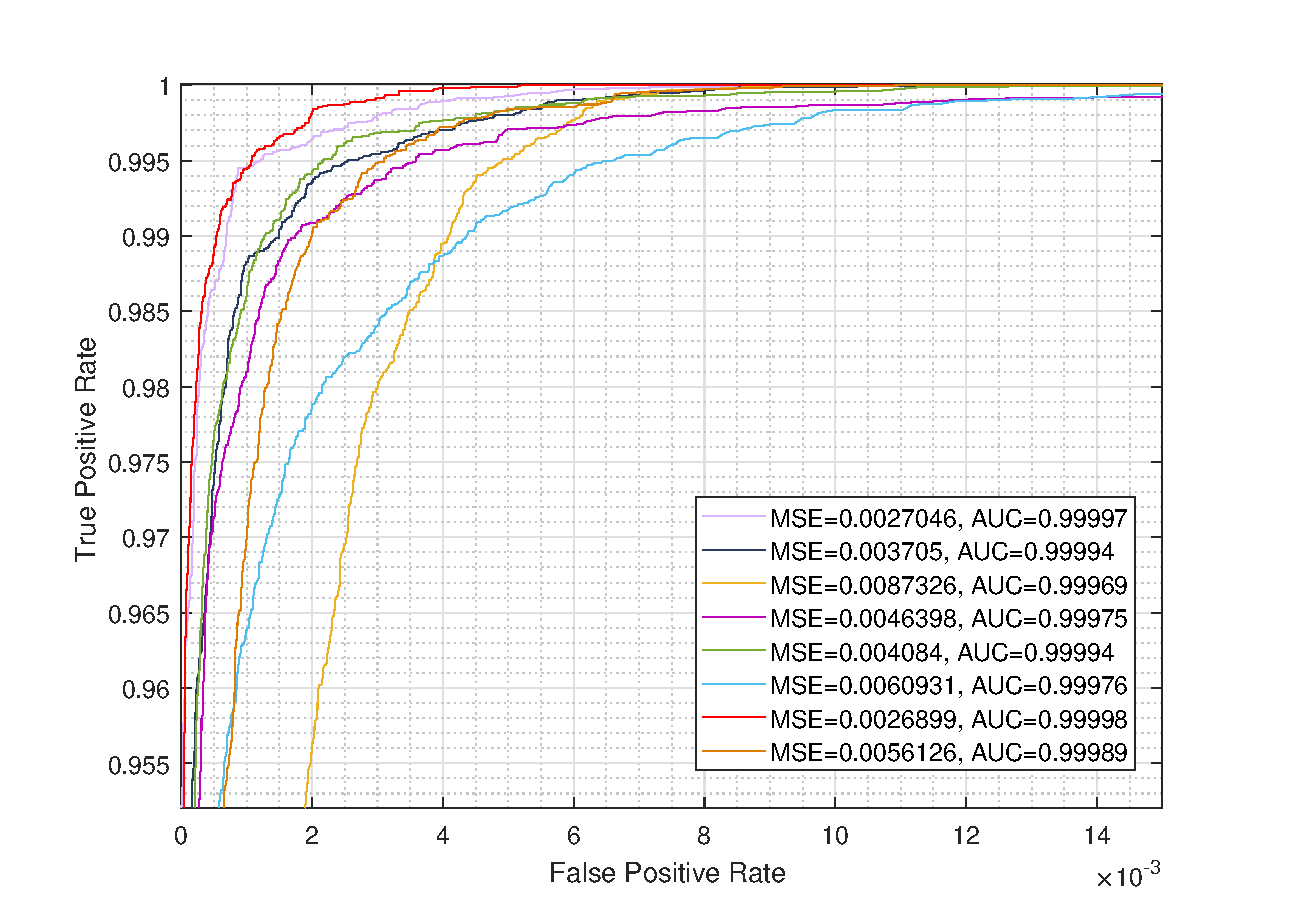
\includegraphics[width=0.5\columnwidth]{mseVSauc.eps}
    \caption{\ac{roc} curves for different BS positions. Lower \ac{mse} are associated to higher \ac{auc}}
    \label{fig:mseVSauc}
\end{figure}

Notice however that the problem is non-convex as the map realization depends on the \acp{bs} position and on a random shadowing and fading realization. Therefore we exploit the \ac{pso} \cite{Kennedy-11}.

\ac{pso} is an iterative optimization algorithm based on social behavior of animals (e.g. birds flocking and fish schools). Consider a particle as a set of positions for the \acp{bs} and consider a total number of $P$ particles. Each one is a possible candidate solution of the optimization problem. Each particle is described by its position $\bm{x}_p$, which is a $N_{\rm BS}$ dimensional vector containing the positions of the \acp{bs} and representing a possible solution, and its velocity $\bm{v}_p$.
Starting from a random initialization of all the particles at each iteration both the positions $\bm{x}_p$ and the velocities $\bm{v}_p$ are updated. Two optimal values are defined in each iteration: the global optimal value found so far by the entire population and a local optimal value for each particle, i.e., the optimal value found by the individual $p$ up to the current iteration. We define as $\bm{o}_g$ the position of the the global optimal values and as $\bm{o}_p$ the position of the optimal value found by particle $p$ at the current iteration.

The position and velocity of the particles are updated at iteration $t$ as
 \begin{equation}\label{eq: v up}
 \bm{v}_p(t) = w\bm{v}_p(t-1)+\phi_1(t)(\bm{o}_p(t-1)-\bm{x}_p(t-1))+\phi_2(t)(\bm{o}_g(t-1)-\bm{x}_p(t-1)), 
 \end{equation}
 \begin{equation}\label{eq: p up}
 \bm{x}_p(t) = \bm{x}_p(t-1) + \bm{v}_p(t),
 \end{equation}
where $w$ is the inertia coefficient and $\phi_1$ and $\phi_2$ are random variables distributed respectively in $[0,c_1]$ and $[0,c_2]$, where $c_1$ and $c_2$ are defined as acceleration constants. The values of the inertia coefficient and of the acceleration constants are the parameters of the \ac{pso} problem. Typical values for this parameters are $w=0.7298$, $c_1=c_2=1.4961$ \cite{Kennedy-11}.

The algorithm steps for \acp{bs} positioning are reported in Algorithm 1. We initialize $P$ particles with random positions for each of the $N_{\rm BS}$ in each particle. For each particle $p$ we then build and train a \ac{nn} and compute the achieved \ac{mse} value MSE$_p^{(0)}$. \ac{pso} is then exploited to iteratively update the position of the particles. Notice that in order to find the best local and global optimal positions \ac{mse} values at the current and previous iterations are compared. If this values are in the same range, i.e., if $|\rm{MSE}_p^{(it-1)}-\rm{MSE}_p^{(it)}|<\lambda_{\rm diff}$ then the \acp{nn}  are also tested and decision is taken based on the \ac{auc} values, otherwise decision is taken based on \ac{mse} values.

\begin{algorithm}[t]
  \algsetup{linenosize=\tiny}
  \scriptsize

 \KwData{ number of particles $P$, $N_{\rm BS}$, $\lambda_{\rm diff}$}
 \KwResult{optimal position }
 Initialization: select random positions for the components of each particle\;
                 build training set for each particle\;
                 build and train a \ac{nn} for each particle and obtain the training performance $\rm{MSE}_p^{(0)}$, $p=1,...,N_p$\;
                 $it = 0$\;

 \Repeat{convergence of particles positions}{
        $it = it + 1$\;
        \For{$p=1,...,P$}{
        update velocity and position vector of particle $p$ via (\ref{eq: v up}) and (\ref{eq: p up})\;
        build a training set\;
        build and test a \ac{nn} and compute $\rm{MSE}_p^{(it)}$\;
        \eIf{$|\rm{MSE}_p^{(it-1)}-\rm{MSE}_p^{(it)}|<\lambda_{\rm diff}$}{
        compute $\rm{AUC}_p^{(it-1)}$ and $\rm{AUC}_p^{(it)}$ for both \acp{nn}\;
        update PSO vectors based on AUC$_p$\;
        
        }{
        update PSO vectors based on MSE$_p$\;
        }
        
        }
      
      }
    
 \caption{BSs positioning algorithm}
\end{algorithm}

The position of the particle that achieves the global minimum \ac{mse} or maximum \ac{auc} at the end of the optimization problem is the best position for the \acp{bs}. Notice that, as the optimization problem is non-convex, solving \ac{pso} is similar to a multi-start  optimization considering $P$ different starting points, which is a standard method used to avoid local minimums. Hence as the number $P$ increases the probability of finding a local solution is reduced.

Notice that the \acp{bs} positioning problem could be solved without implementing a \ac{nn} by mean of computation of the \acp{llr} for the different positions. However we showed in Section \ref{sec:shadow} that when considering multiple \acp{bs} and including shadowing effects the exact computation of the \ac{llr} curve requires more data than those needed for training a \ac{nn}. Hence the proposed solution is effective in terms of both authentication performance and number of needed data.

\section{Attack strategies}
The proposed techniques can be exploited in order to provide not only an authentication system, but also for implementing an attack strategy. The idea is here to use attenuation values measured from the non-authentic area and to train a \ac{ml} architecture based on these values.

The first architecture we exploit is the \ac{rnn}. The \ac{rnn} is here trained in order to reproduce at the output attenuation vectors measured from the non-authentic area. We propose two attack strategies: a random generation attack and a manifold based attack.

\subsection{Random generation attack}
After that the \ac{rnn} has been trained with attenuation vectors measured from the non-authentic area, only attenuation vectors with the same statistical structure will be reproduced at the output with a reconstruction error $\epsilon$ (\ref{eq: rec err}) lower than $\gamma$. The idea is hence to generate a random attenuation vector $\bm{a}_{\rm test}$ and to feed it to the \ac{rnn}: if the output has a reconstruction error lower than $\gamma$ then $\bm{a}_{\rm test}$ is considered as belonging to the non-authentic area, otherwise the it is considered as a possible candidate for a successful attack. This vector is hence tested and, if the attack is not successful, we label it as belonging to the non-authentic area.

As new randomly generated vectors are not successful or have a reconstruction error lower than $\gamma$ we gain information about the structure of the non-authentic area. We hence update the \ac{rnn} training in a mini-batch fashion when a sufficient number of new vectors (good results can be achieved with batch size of $m=3$ or $m=4$ new vectors per update \cite{bengio-12}) is obtained. These vectors are stored in matrix $\bm{A}_{\rm test}$ and when $m$ vectors populate the matrix mini-batch gradient descent is executed on the \ac{rnn} to update its parameters.

The algorithm steps are reported in Algorithm 2.

\begin{algorithm}[t]
  \algsetup{linenosize=\tiny}
  \scriptsize

 \KwData{ weight and bias vectors of the trained RNN}
 \KwResult{authentic attenuation vector }
 

 \Repeat{authentic attenuation vector has been obtained}{
        generate random attenuation vector $\bm{a}_{\rm test}$\;
        compute reconstruction error $\epsilon$ of $\bm{a}_{\rm test}$ via (\ref{eq: rec err})\;
        \eIf{$\epsilon < \gamma$}{$\bm{a}_{\rm test}$ belongs to non-authentic area\;
        store $\bm{a}_{\rm test}$ in $\bm{A}_{\rm test}$\;}
        {test $\bm{a}_{\rm test}$ for an attack\;
        \eIf{attack is successful}{return $\bm{a}_{\rm test}$}
        {store $\bm{a}_{\rm test}$ in $\bm{A}_{\rm test}$\;}
        }
        \If{size($\bm{A_{\rm test}}) = m$}{update RNN training via mini-batch gradient descent\;
        delete vectors from $\bm{A}_{\rm test}$\;}
      
      }
    
 \caption{Random generation attack}
\end{algorithm}


\subsection{Manifold based attack}
The second attack strategy exploits the encoding properties of the \ac{rnn}. Consider an optimal-compression \ac{rnn} \cite{hecht-95} and let $\Phi:[0,1]^M \to \mathbb{D}$ be a smooth orientation-preserving diffeomorphism of the unit cube $[0,1]^M \subset \mathbb{R}^M$ onto the data manifold $\mathbb{D} \subset \mathbb{R}^N$. The natural coordinates of a point $\bm{x}$ on $\mathbb{D}$ are defined as the Cartesian coordinates of its pre-image $\Phi^{-1}(\bm{x})$ on the cube. From the theorem in \cite{hecht-95} we know that a \ac{rnn} configured to perform a reconstruction of a value on the data manifold $\mathbb{D}$ within a \ac{mse} $\epsilon$ outputs at the hidden layer neurons the natural coordinates of the given input.

This allows us to construct the manifold of the non-authentic area and hence to generate data that are certainly out of the training area, reducing hence the time needed to generate vectors that do not have the same characteristics of those used for training.

In order to build the manifold of the training set we compute the outputs of the hidden layer when the vectors of the training set are fed as input. 

\section{Numerical results: los scenario}\label{sec:res_los}
In order to confirm the theoretical results obtained so far and compare the different solutions we test the performance of the authentication systems based on two measures: the \textit{true positive rate} and the \textit{false positive rate}. 

Let us define as \textit{true positive} the number of \acp{ue} located in area $\mathcal{A}_0$ which are considered in area $\mathcal{A}_0$ by the authentication system, whereas we define as \textit{false positive} the number of \acp{ue} located in area $\mathcal{A}_1$ which are considered in area $\mathcal{A}_0$ by the authentication system. Furthermore let us define as \textit{true negative} the number of \acp{ue} located in area $\mathcal{A}_1$ which are considered in area $\mathcal{A}_1$ by the authentication system, whereas we define as \textit{false negative} the number of \acp{ue} located in area $\mathcal{A}_0$ which are considered in area $\mathcal{A}_1$ by the authentication system.
We hence define the true positive rate as
\begin{equation}
    \text{true positive rate} = \frac{\text{true positive}}{\text{ true positive + false negative}};
\end{equation}
and the false positive rate as
\begin{equation}
    \text{false positive rate} = \frac{\text{false positive}}{\text{false positive + true negative}},
\end{equation}

Consider the \ac{los} scenario. Let us define the overall network area as a circle $\mathcal{C}$ with radius $R_{\rm out}$ and consider a single \ac{bs} located at the center of $\mathcal{C}$. Consider the legitimate area $\mathcal{A}_{0}$ as a rectangle of height $H$ and length $L$ and with nearest point to the center of $\mathcal{C}$ at a distance $R_{\rm min}$. The non-legitimate area is $\mathcal{A}_1 = \mathcal{C} \setminus \mathcal{A}_0$.

Since we stated that in the \ac{los} scenario the attenuation incurred by a \ac{ue} only depends on its relative distance to the \ac{bs} we can here compute a closed form solution for the \ac{llr} in (\ref{eq:lr}) and hence compare the machine learning-based solutions to the \ac{np} classification.

Consider a \ac{ue} $u$ transmitting a message to the \ac{bs} located at a distance $R_0$ from the \ac{bs}. The probability othat $u$ is located at a distance $R\le R_0$ in $\mathcal{A}_0$ is
\begin{equation}\label{eq:cdf}
     \mathbb{P}(R \le R_0|\mathcal{A}_0) = \frac{1}{|\mathcal{A}_0|}\int_{R_{\rm min}}^{R_0} R a(R) dR,
\end{equation}
where $a(R)$ denotes the angle of the circular sector located at distance $R$ intersecting area $\mathcal{A}_0$.

By taking the derivative of (\ref{eq:cdf}) respect to $R_0$ we obtain the \ac{pdf} of $u$ transmitting from a distance $R_0$ given that it is located in $\mathcal{A}_0$ as
\begin{equation}
    p(R_0|\mathcal{A}_0) = \frac{1}{|\mathcal{A}_0|}R_0a(R_0).
\end{equation}
Following the same reasoning and considering that the length of the arc of circle with radius $R_0$ located in $\mathcal{A}_1$ is $2\pi - a(R_0)$, we obtain the \ac{pdf} of $u$ being at a distance $R_0$ given that it is located in $\mathcal{A}_1$ as
\begin{equation}
     p(R_0|\mathcal{A}_1) = \frac{1}{|\mathcal{A}_1|}R_0\left(2\pi-a(R_0)\right),
\end{equation}
from which we obtain the closed form solution for (\ref{eq:lr}) 
\begin{equation}
    \mathcal{L}=\log\left(\frac{|\mathcal{A}_1|a(R_0)}{|\mathcal{A}_0|\left(2\pi-a(R_0)\right)}\right),
\end{equation}

The attenuation value measured at the \ac{bs} for a user is given by (\ref{eq:los}), where we consider a unitary transmitting power for each user and a carrier frequency of $2.12$ GHz.
\begin{figure}[h]
    \centering
    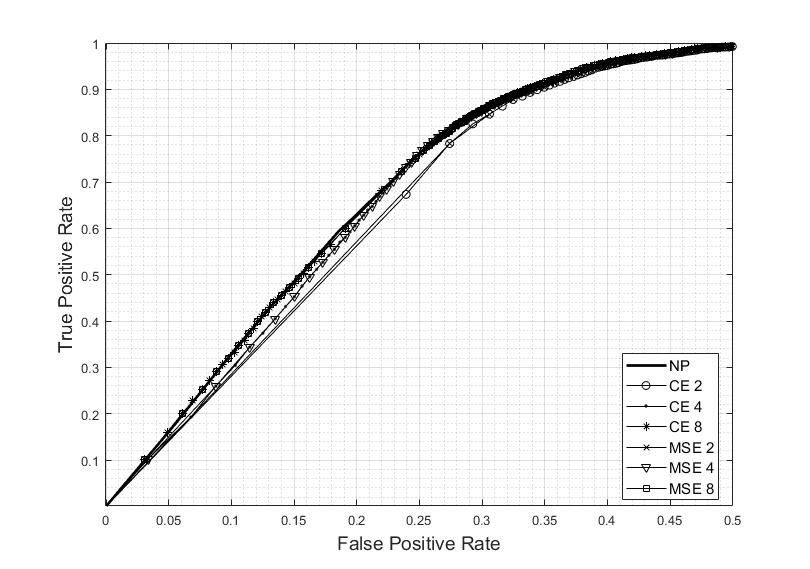
\includegraphics[width=0.5\columnwidth]{mseVSce.jpg}
    \caption{True positive rate vs. false positive rate obtained in the LOS scenario with a single BS. Comparison between NP detector, MLP with MSE training and MLP with CE training with different number of neurons in the hidden layer.}
    \label{fig:ceVSmse}
\end{figure}

Fig. \ref{fig:ceVSmse} show the true positive rate vs. false positive rate obtained by the authentication system with $10^5$ training points and $10^5$ testing points. In particular we here compare the performance of the \ac{np} detector with the \ac{ce}-trained and with the \ac{mse}-trained \acp{mlp}. Furthermore we show the performance of the \acp{mlp} when the hidden layer is composed by $2,4 $ and $8$ neurons. We first notice that the \ac{ce}-trained and \ac{mse}-trained \acp{mlp} obtain the same performance when considering the same number of neurons in the hidden layer. This confirms that the two training methods are performing hypothesis testing in an equivalent manner. Furthermore we notice that as the number of neurons at the hidden layer grows the performance of the \ac{mlp} classificators approach those obtained by the \ac{np} classificator, up to the point where they are the same with $8$ neurons. This shows that both \ac{ce}-trained and \ac{mse}-trained \acp{mlp} are performing the optimal \ac{np} test and that convergence is obtained with a small number of neurons.



\section{Numerical results: non-los scenario}\label{sec:res_nLos}
\subsection{Shadowing effects}\label{sec:shadow}
In this section we consider the non-\ac{los} scenario and we show that the \ac{ml}-based solutions are convenient over the \ac{np}-based one.

Fig. \ref{fig:map} shows a realization of the attenuation map. A spatial grid has been created in order to take into account the shadowing's spatial correlation over different locations in space. The network includes a single \ac{bs} located at the map center and a squared authentic area $\mathcal{A}_0$, delimited in figure by the red line. Furthermore we consider two \ac{los} paths, one parallel to the $x$ axis and one parallel to the $y$ axis and intersecting at the map center.

Consider the \ac{llr} (\ref{eq:lr}). In the non-\ac{los} context the computation of the two area dependent probabilities has no closed-form solution. A numerical solution is obtained by sampling the attenuation values over the spatial grid of positions. Consider an attenuation value $\hat{a}$: the probability of measuring $\hat{a}$ given that the \ac{ue} is located in area $\mathcal{A}_0$ is given by the number of positions $(x_u,y_u)$ inside $\mathcal{A}_0$ where the measured attenuation $a(x_u,y_u)=\hat{a}$ over the total number of positions $(x_u,y_u)$ in the entire map with the same attenuation $\hat{a}$, i.e.
\begin{equation}
    \mathbb{P}(\hat{a}|\mathcal{A}_0) \approx \frac{\text{number of positions} \, (x_u,y_u) \in \mathcal{A}_0 \, \text{s.t.} \, a(x_u,y_u) = \hat{a}}{\text{total number of positions} \, (x_u,y_u) \, \text{s.t.} \, a(x_u,y_u) = \hat{a}}
\end{equation}
An approximation of equation (\ref{eq:lr} is hence obtained as
\begin{equation}\label{eq:lrApp}
    \mathcal{L} \approx \frac{\text{number of positions} \, (x_u,y_u) \in \mathcal{A}_0 \, \text{s.t.} \, a(x_u,y_u) = \hat{a}}{\text{number of positions} \, (x_u,y_u) \in \mathcal{A}_1 \, \text{s.t.} \, a(x_u,y_u) = \hat{a}}
\end{equation}
The approximation gets closer to the real value as the number of grid points over the map increases, as an higher number of points means a better statistical characterization of the attenuation over the map area.

Fig. \ref{fig:trueMap} shows the true positive rate vs. the false positive rate obtained for the attenuation map in Fig. \ref{fig:map}. In particular we here compare the results obtained with approximation (\ref{eq:lrApp}) with the results obtained with the \ac{mse} trained \ac{mlp} with different number of neurons in the hidden layer.
For the computation of (\ref{eq:lrApp}) we built a grid with $4.46 \cdot 10^6$ space points, whereas for training and testing the \ac{mlp} we used respectively $10^5$ and $10^6$ points. We notice that the \ac{mlp} achieves better results than the \ac{np}-based detector. This means that the considered number of grid points is not sufficient to approximate the optimal \ac{np} solution. Furthermore we tested the \ac{mlp} with $1,3$ and $10$ neurons at the hidden layer. We see that the performance with $1$ and $3$ neurons are the same, whereas with $10$ neurons we achieve the \ac{np} solution, based on the results of the previous section. 

Comparing the number of grid points and the number of training points used for the \ac{mlp} we can hence conclude that the \ac{mlp}-based solution is advantageous over the \ac{np}-based one, as it requires a smaller number of points to achieve the optimal solution. Furthermore this implies that the \ac{mlp}-based authentication system can be implemented without a-priory knowledge of the \ac{pdf} of the hypothesis to be tested.

Consider the network in Fig. \ref{fig:mBS}. $N_{\rm bs}=5$ \acp{bs} gather attenuation values from the \acp{ue}. Each \ac{bs} has its own attenuation map given by path loss, shadowing and fading realization. Each \ac{bs} gathers the attenuation value of the transmitting \ac{ue} and sends it to the central unit, which builds the attenuation vector $\bm{a}$ that is used for discriminating the location of the considered \ac{ue}.

Fig. \ref{fig:rnnMLP} compares the performance of the \ac{mlp}-based solution with those of the \ac{rnn}-based solution. Results have been obtained for the network configuration in Fig. \ref{fig:mBS}. Both architectures have been trained over a set of $10^5$ attenuation vectors and tested over the same set of $10^5$ attenuation vectors. Notice that the training set of the \ac{mlp} comprises attenuation vectors measured in both $\mathcal{A}_0$ and $\mathcal{A}_1$. The \ac{mlp} is trained with \ac{mse} loss function and we compare the results obtained with a number of neurons in the hidden layer from $1$ to $5$. The performance of the \ac{rnn}-based solution are here presented for a number of neurons in the hidden layer from $1$ to $5$. Both architectures are composed by an input layer, a hidden layer and an output layer. Curves for the \ac{mlp} are obtained by varying the threshold value $\lambda$, whereas for \ac{rnn} are obtained by varying the threshold value $\gamma$. We notice that the performance of the \ac{rnn} with £4£ neurons in the hidden layer are better compared to those obtained with the \ac{rnn} with $4$ and $5$ neurons in the hidden layer. This is due to the fact that the features extracted by $3$ neurons in the hidden layer better represent data in $\mathcal{A}_0$, whereas $4$ and $5$ neurons are over-representative. This confirms that the feature extraction process of the \ac{rnn} is an efficient way to represent a set. We further notice that the performance of the \ac{rnn} with $2$ neurons in the hidden layer are worse than those obtained with the \ac{rnn} with $3$ neurons in the hidden layer. This is due to the fact that $2$ neurons are not sufficient for the feature extraction process to provide a good characterization of area $\mathcal{A}_0$. We notice that the performance obtained with the \ac{mlp}-solution are better than those obtained with the \ac{rnn}. 

\begin{figure}
    \centering
    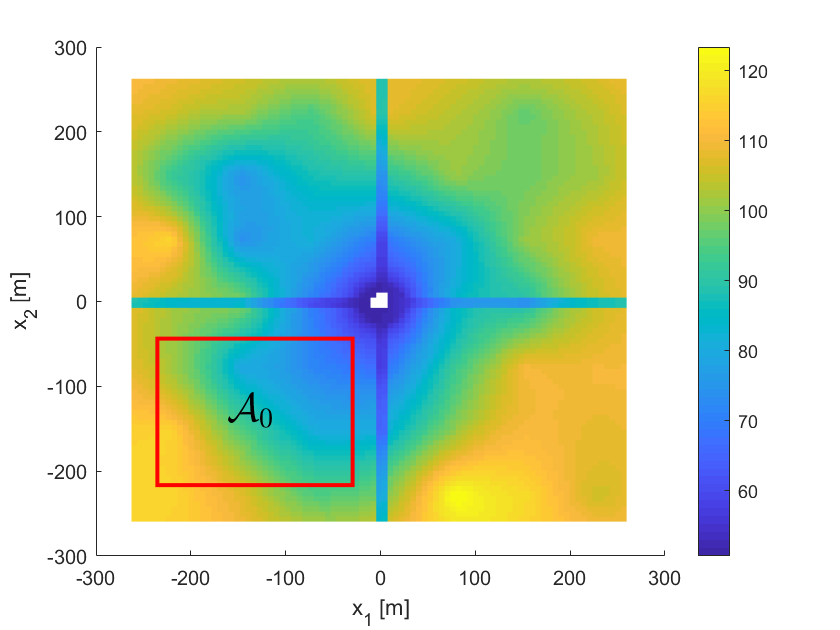
\includegraphics[width=0.5\columnwidth]{surfColorato.png}
    \caption{Example of a realization of the attenuation map in the non-\ac{los} scenario considering only the shadowing effects.}
    \label{fig:map}
\end{figure}


\begin{figure}
    \centering
    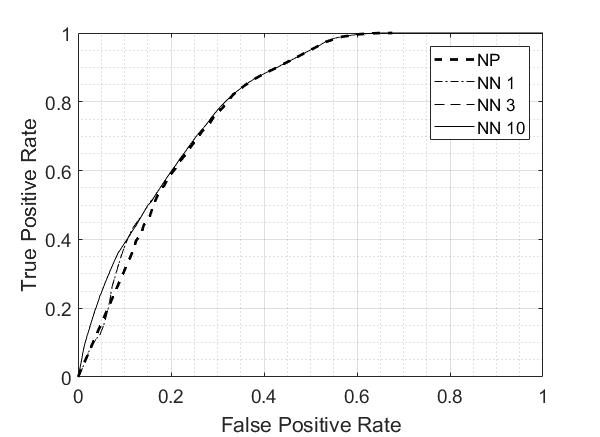
\includegraphics[width=0.5\columnwidth]{trueMap.jpg}
    \caption{True positive rate vs. false positive rate for the attenuation map in Fig. \ref{fig:map}. Comparison between the \ac{np}-based and the \ac{mlp}-based detectors}
    \label{fig:trueMap}
\end{figure}

\begin{figure}
    \centering
    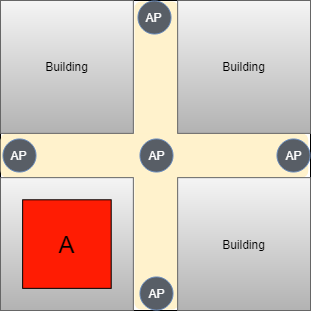
\includegraphics[width=0.3\columnwidth]{scenario2.png}
    \caption{Scenario with multiple BSs: each one gathers the attenuation value of the transmitting user and passes it to the central unit that builds the attenuation vector $\bm{a}$ used for discriminating the location of the user.}
    \label{fig:mBS}
\end{figure}

\begin{figure}
    \centering
    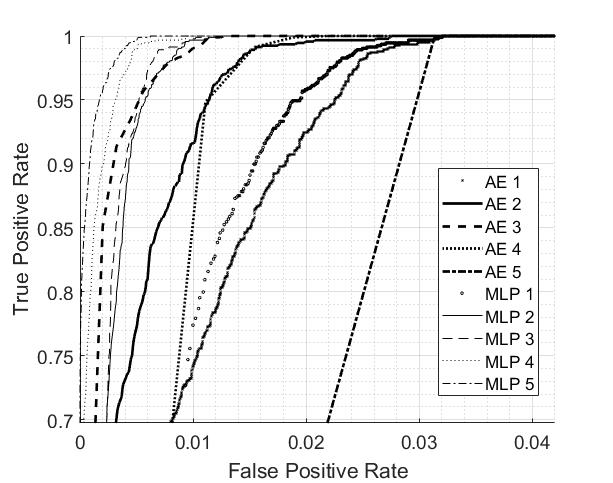
\includegraphics[width=0.5\columnwidth]{RNNvsMLPnNeur.jpg}
    \caption{True positive rate vs. false positive rate for the network configuration in Fig. \ref{fig:mBS}. Comparison between the \ac{mlp}-based and the \ac{rnn}-based detectors with different number of neurons in the hidden layer.}
    \label{fig:rnnMLP}
\end{figure}


\subsection{Fading effects}
Let us now include the fading effects. The attenuation in point $(x_u,y_u)$ is a Gaussian random variable with zero mean and variance given by the inverse of the value of the map in $(x_u,y_u)$.


In order to compute the \ac{llr} in (\ref{eq:lr}) we should here consider a $N_{\rm bs}$-dimensional multivariate Gaussian distribution. However, as this equation has no closed-form solution and we showed in \ref{sec:shadow} that the \ac{mlp}-based solution achieves the optimal results of the \ac{np} detector with fewer points we implement the \ac{mlp}-based solution. A larger number of \acp{bs} means a larger feature space to be fed to the \ac{mlp}. We hence expect that the performance of the system increase with the number of \acp{bs}.

Different fading realizations lead to different statistical characterization of the attenuation values measured in both areas. Therefore training the \ac{mlp} over a single fading realization could lead to a non-optimal result in the successive realization. We hence propose to train and test the \ac{mlp} over $N_{\rm avg}$ fading realizations for each \ac{bs}.

Fig. \ref{fig:faded} shows the true positive rate vs. the false positive rate in non-\ac{los} scenario with fading effects. Different number of fading realizations for training a \ac{mlp} with \ac{mse} loss function has been considered. We notice that as the number $N_{\rm avg}$ of fading realizations used for training increases the performance of the network get closer to those obtained without considering the fading effects. Furthermore we notice that, as expected, with a larger number of \acp{bs} the performance of the system increase, as can be seen comparing the curve in Fig. \ref{fig:trueMap} and the 'No fading' curve in Fig. \ref{fig:faded}.

\begin{figure}
    \centering
    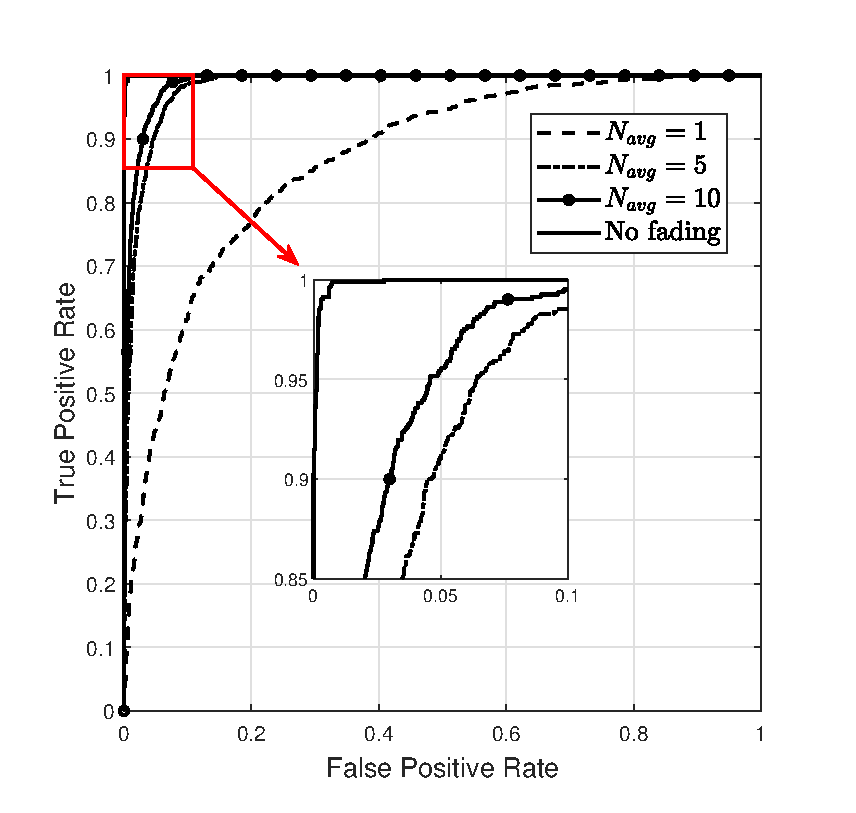
\includegraphics[width=0.5\columnwidth]{Navg.eps}
    \caption{True positive rate vs. false positive rate in non-LOS scenario with fading effects. Comparison between training with different number of fading realizations.}
    \label{fig:faded}
\end{figure}
\newpage 




\bibliographystyle{IEEEtran}
\bibliography{bibliography.bib}
\end{document}
